\documentclass[a4paper,12pt]{article}
\usepackage[utf8]{inputenc}
\usepackage[ngerman]{babel}
\usepackage{graphicx}
\usepackage{amsmath}
\usepackage{hyperref}

\title{Analyse der Bevölkerungsentwicklung in Tirol}
\author{Luna Schäzle}
\date{\today}

\begin{document}

\maketitle

\tableofcontents
\newpage

\section{Einleitung}

In dieser Analyse wird die Bevölkerungsentwicklung in Tirol, Innsbruck und verschiedenen Bezirken untersucht. Ziel ist es, historische Entwicklungen darzustellen, Prognosen für die Zukunft zu erstellen und Vergleiche zwischen verschiedenen Regionen zu ziehen. Die verwendeten Daten stammen aus einer CSV-Datei, und für die Umsetzung wurden die Python-Bibliotheken \texttt{pandas}, \texttt{matplotlib} und \texttt{statsmodels} eingesetzt.

\section{Aufgabe 1: Daten einlesen}

Die Bevölkerungsdaten werden aus der Datei \texttt{bev\_tirol.csv} eingelesen. Die Daten umfassen die Bevölkerungszahlen von Tirol, Innsbruck und verschiedenen Bezirken. Der folgende Python-Code zeigt, wie die Daten eingelesen wurden:

\begin{verbatim}
import pandas as pd
import matplotlib.pyplot as plt
import statsmodels.api as sm

data = pd.read_csv("bev_tirol.csv", sep=";")
\end{verbatim}

\section{Aufgabe 2: Bevölkerungsentwicklung in Tirol}

\subsection{Bevölkerungsentwicklung}

Die Bevölkerungsentwicklung in Tirol von 1990 bis 2022 wird analysiert. Ein Liniendiagramm zeigt den Verlauf der Gesamtbevölkerung über die Jahre (siehe Abbildung \ref{fig:tirol-entw}).

Aus dem Diagramm ist ein mehr oder weniger konstanter Anstieg der Bevölkerung in Tirol erkennbar. Dieser langfristige Trend deutet auf ein stetiges Bevölkerungswachstum hin.

\subsection{Prognose}

Anhand der historischen Daten wurde eine Prognose für die Bevölkerungsentwicklung bis ins Jahr 2030 erstellt. Dabei wurde ein lineares Regressionsmodell verwendet (siehe Abbildung \ref{fig:tirol-prognose}).

Die Prognose zeigt, dass die Bevölkerung in Tirol weiterhin steigen wird, wenn der aktuelle Trend anhält. Prognosen sollten jedoch mit Vorsicht betrachtet werden, da unvorhergesehene Ereignisse oder geografische Einschränkungen die Entwicklung beeinflussen können.

\section{Aufgabe 3: Bevölkerungsentwicklung in Innsbruck}

\subsection{Bevölkerungsentwicklung in Innsbruck}

Für Innsbruck wurde die Bevölkerungsentwicklung separat analysiert. Ein allgemeiner Aufwärtstrend ist erkennbar, jedoch mit stärkeren Schwankungen (siehe Abbildung \ref{fig:innsbruck-entw}).

Im Vergleich zu Tirol sind die Schwankungen in Innsbruck deutlicher ausgeprägt. Besonders in den letzten Jahren gab es Rückgänge, die auf verschiedene Faktoren wie Abwanderung oder Veränderungen der Wohnsituation zurückzuführen sein könnten.

\subsection{Prognose}

Für Innsbruck wurde ebenfalls eine Prognose bis zum Jahr 2030 erstellt (siehe Abbildung \ref{fig:innsbruck-prognose}).

Die Prognose deutet darauf hin, dass die Bevölkerungszahl in Innsbruck weiter steigen könnte, sofern sich der Rückgang der letzten Jahre nicht fortsetzt.

\section{Aufgabe 4: Gegenüberstellung der Bezirke}

Für die Bezirke Innsbruck-Land (IL) und Kufstein (KU) wurde die Bevölkerungsentwicklung gegenübergestellt, um Unterschiede und Gemeinsamkeiten zu identifizieren (siehe Abbildung \ref{fig:bezirk-vergleich}).

Die Bevölkerungsentwicklung in beiden Bezirken zeigt ähnliche Muster. Die Schwankungen verlaufen in ähnlichen Jahren, was auf gemeinsame externe Faktoren hinweisen könnte. Kufstein hat jedoch eine geringere Gesamtbevölkerung im Vergleich zu Innsbruck-Land, während beide Bezirke ein vergleichbares Wachstumsmuster aufweisen.

\section{Fazit}

Die Analyse zeigt, dass Tirol insgesamt ein stetiges Bevölkerungswachstum verzeichnet. Innsbruck als urbanes Zentrum weist eine dynamischere Entwicklung mit stärkeren Schwankungen auf, während die Bezirke Innsbruck-Land und Kufstein ein ähnliches Wachstumsmuster zeigen. Prognosen bis 2030 deuten auf eine Fortsetzung des Wachstums hin, wobei externe Einflüsse und geografische Gegebenheiten berücksichtigt werden sollten.

\section{Quellcode}

Der vollständige Quellcode zu dieser Auswertung ist auf GitHub verfügbar:
\begin{itemize}
    \item \url{https://github.com/Luna-Schaetzle/INFI_Informations_Systeme/tree/main/Uebung_4}
\end{itemize}

\newpage
\section{Abbildungen}

\begin{figure}[h]
    \centering
    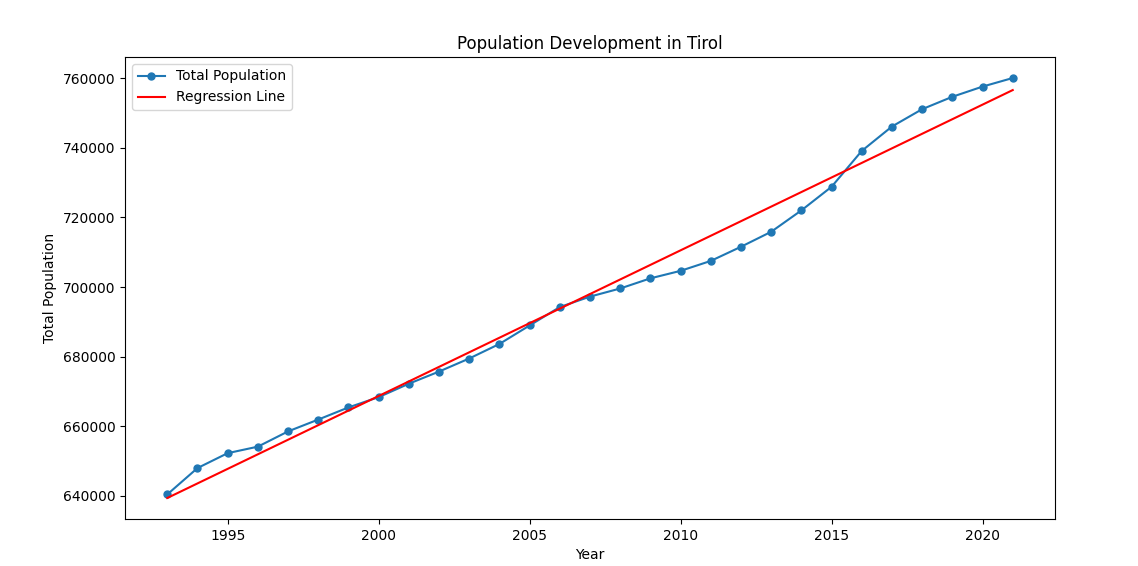
\includegraphics[width=\textwidth]{image.png}
    \caption{Bevölkerungsentwicklung von 1990 bis 2022 für ganz Tirol.}
    \label{fig:tirol-entw}
\end{figure}

\begin{figure}[h]
    \centering
    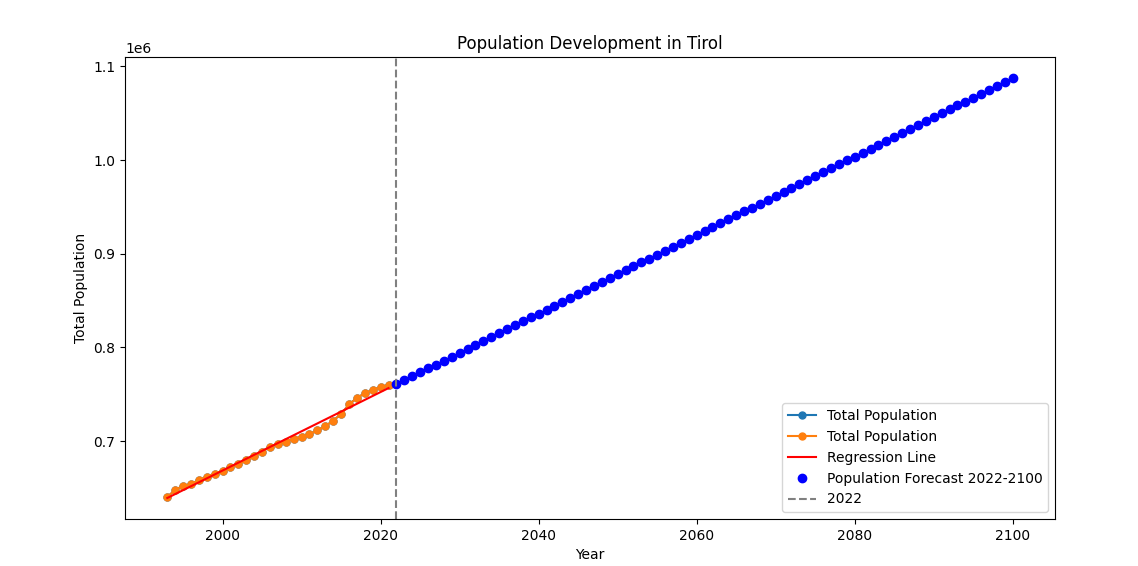
\includegraphics[width=\textwidth]{image-1.png}
    \caption{Prognose der Bevölkerungsentwicklung bis 2100 für Tirol.}
    \label{fig:tirol-prognose}
\end{figure}

\begin{figure}[h]
    \centering
    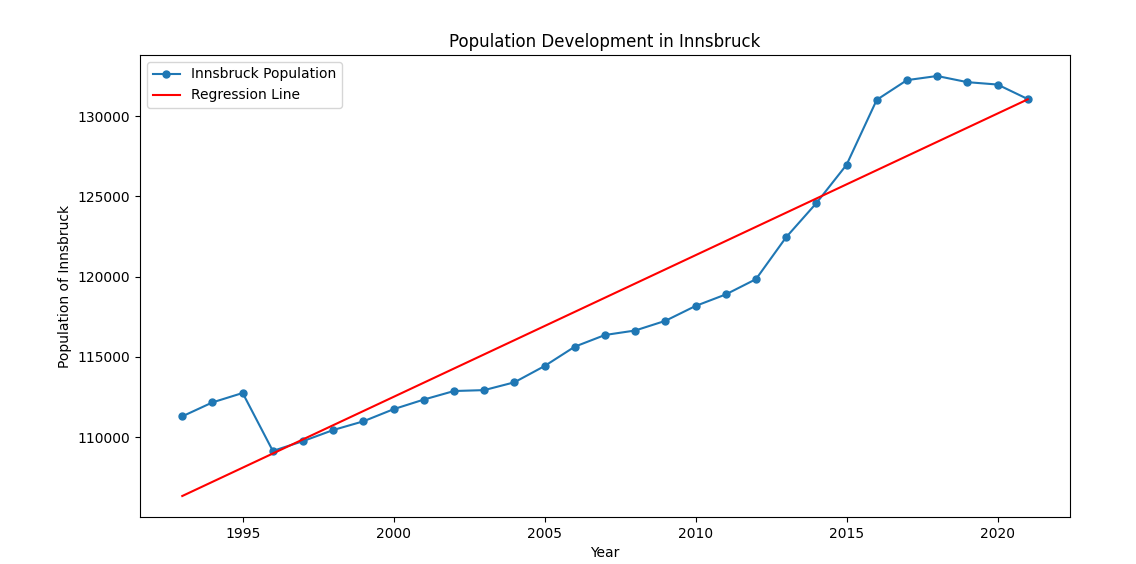
\includegraphics[width=\textwidth]{image-2.png}
    \caption{Bevölkerungsentwicklung für Innsbruck.}
    \label{fig:innsbruck-entw}
\end{figure}

\begin{figure}[h]
    \centering
    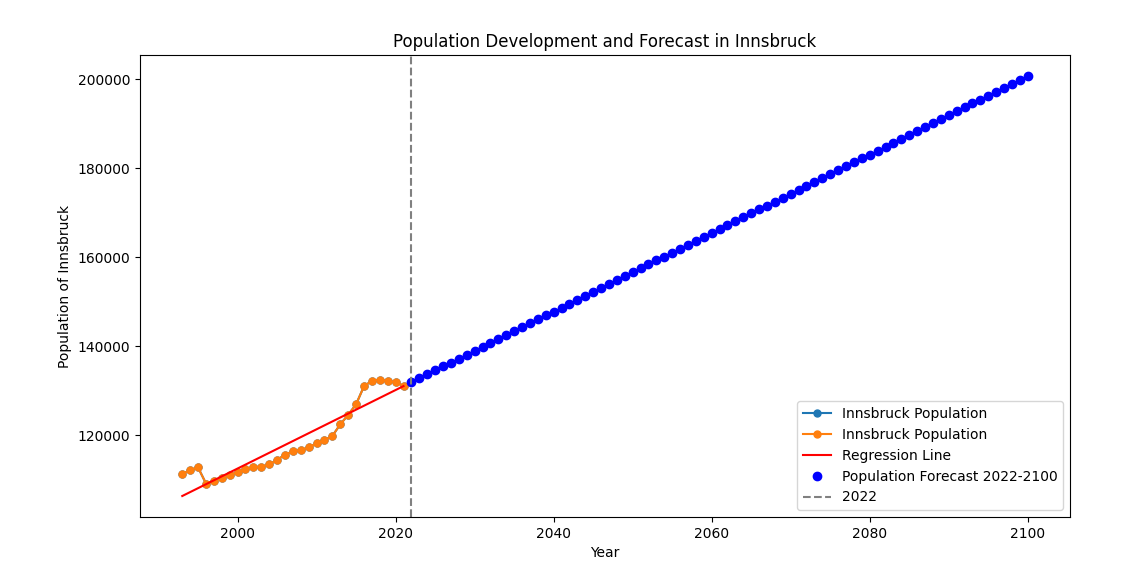
\includegraphics[width=\textwidth]{image-3.png}
    \caption{Prognose der Bevölkerungsentwicklung bis 2100 für Innsbruck.}
    \label{fig:innsbruck-prognose}
\end{figure}

\begin{figure}[h]
    \centering
    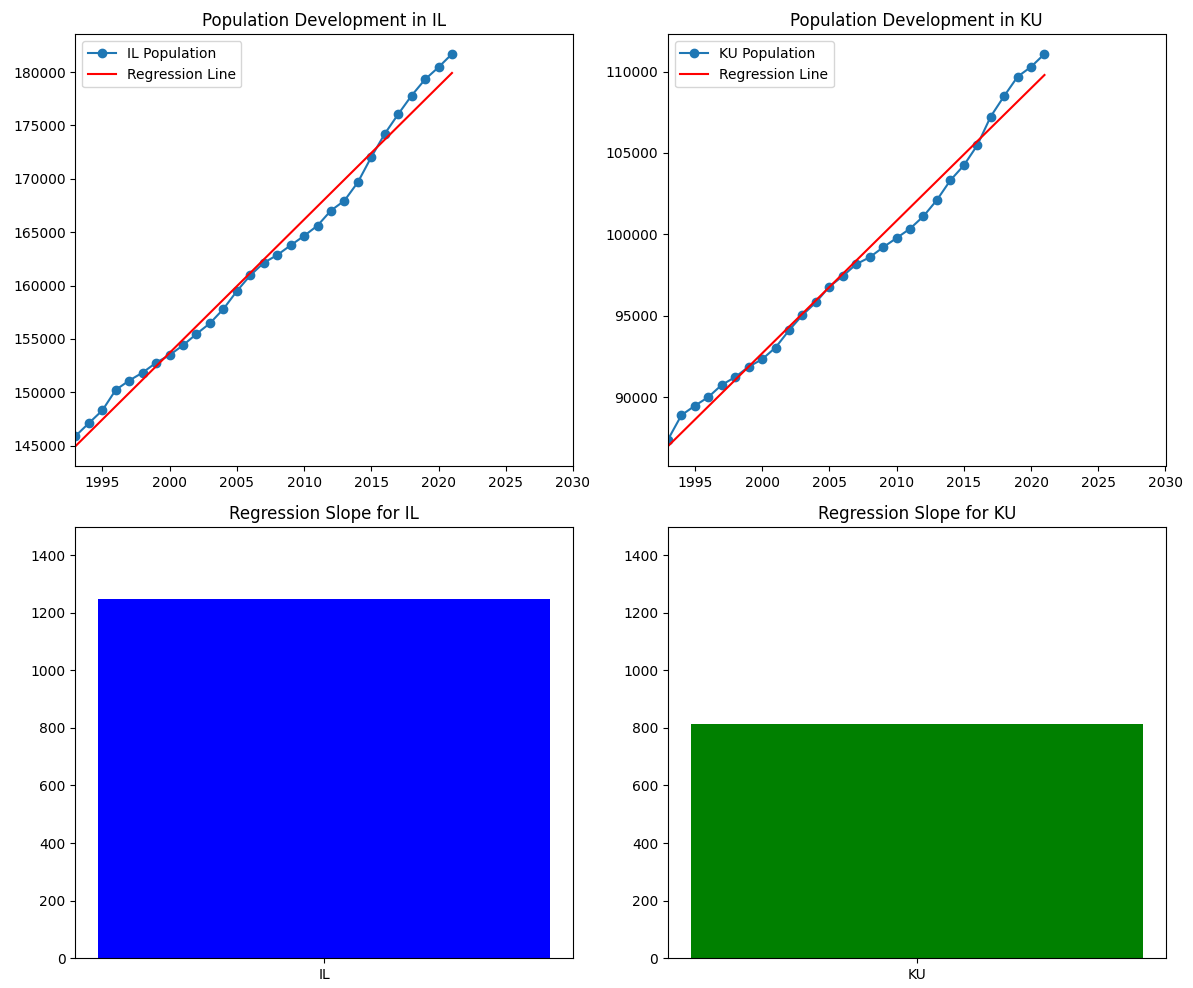
\includegraphics[width=\textwidth]{image-4.png}
    \caption{Vergleich der Bezirke Innsbruck-Land und Kufstein.}
    \label{fig:bezirk-vergleich}
\end{figure}

\end{document}
